\begin{figure}[t]
    \centering
    \begin{minipage}[t]{0.48\textwidth}
        \centering
        % trim={<left> <lower> <right> <upper>}
        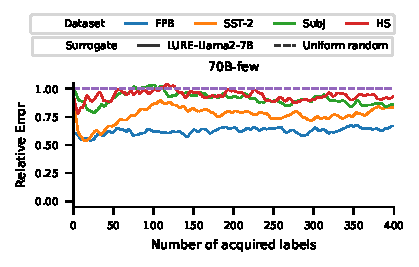
\includegraphics[width=\linewidth,trim={0 5pt 0 0}]{
            figures/pdf/70b_fewshot_entropy_relative_error.pdf
        }
        \caption{
            Using the surrogate model to approximate the target model during data acquisition (here this means acquiring data based on the predictive entropy of the surrogate model) reduces the need for target-model predictions while still performing well.
        }
        \label{fig:70b_fewshot_entropy_relative_error}
    \end{minipage}
    \hfill
    \begin{minipage}[t]{0.48\textwidth}
        \centering
        % trim={<left> <lower> <right> <upper>}
        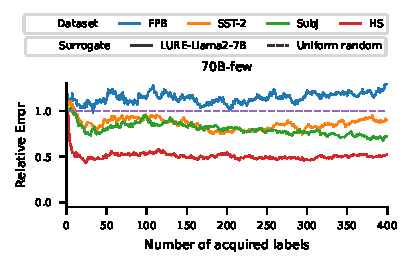
\includegraphics[width=\linewidth,trim={0 5pt 0 0}]{
            figures/pdf/70b_fewshot_nll_relative_error.pdf
        }
        \caption{
            Active testing with a label-aware acquisition function (here the negative log likelihood of the surrogate model) enables dataset curation (selecting a subset of already-labelled test data) tailored to a target model of interest, helping reduce computational costs.
        }
        \label{fig:70b_fewshot_nll_relative_error}
    \end{minipage}
    \vspace{-5pt}
\end{figure}